\documentclass[twoside]{book}

% Packages required by doxygen
\usepackage{fixltx2e}
\usepackage{calc}
\usepackage{doxygen}
\usepackage[export]{adjustbox} % also loads graphicx
\usepackage{graphicx}
\usepackage[utf8]{inputenc}
\usepackage{makeidx}
\usepackage{multicol}
\usepackage{multirow}
\PassOptionsToPackage{warn}{textcomp}
\usepackage{textcomp}
\usepackage[nointegrals]{wasysym}
\usepackage[table]{xcolor}

% NLS support packages
\usepackage[brazil]{babel}
% Font selection
\usepackage[T1]{fontenc}
\usepackage[scaled=.90]{helvet}
\usepackage{courier}
\usepackage{amssymb}
\usepackage{sectsty}
\renewcommand{\familydefault}{\sfdefault}
\allsectionsfont{%
  \fontseries{bc}\selectfont%
  \color{darkgray}%
}
\renewcommand{\DoxyLabelFont}{%
  \fontseries{bc}\selectfont%
  \color{darkgray}%
}
\newcommand{\+}{\discretionary{\mbox{\scriptsize$\hookleftarrow$}}{}{}}

% Page & text layout
\usepackage{geometry}
\geometry{%
  a4paper,%
  top=2.5cm,%
  bottom=2.5cm,%
  left=2.5cm,%
  right=2.5cm%
}
\tolerance=750
\hfuzz=15pt
\hbadness=750
\setlength{\emergencystretch}{15pt}
\setlength{\parindent}{0cm}
\setlength{\parskip}{3ex plus 2ex minus 2ex}
\makeatletter
\renewcommand{\paragraph}{%
  \@startsection{paragraph}{4}{0ex}{-1.0ex}{1.0ex}{%
    \normalfont\normalsize\bfseries\SS@parafont%
  }%
}
\renewcommand{\subparagraph}{%
  \@startsection{subparagraph}{5}{0ex}{-1.0ex}{1.0ex}{%
    \normalfont\normalsize\bfseries\SS@subparafont%
  }%
}
\makeatother

% Headers & footers
\usepackage{fancyhdr}
\pagestyle{fancyplain}
\fancyhead[LE]{\fancyplain{}{\bfseries\thepage}}
\fancyhead[CE]{\fancyplain{}{}}
\fancyhead[RE]{\fancyplain{}{\bfseries\leftmark}}
\fancyhead[LO]{\fancyplain{}{\bfseries\rightmark}}
\fancyhead[CO]{\fancyplain{}{}}
\fancyhead[RO]{\fancyplain{}{\bfseries\thepage}}
\fancyfoot[LE]{\fancyplain{}{}}
\fancyfoot[CE]{\fancyplain{}{}}
\fancyfoot[RE]{\fancyplain{}{\bfseries\scriptsize Gerado por Doxygen }}
\fancyfoot[LO]{\fancyplain{}{\bfseries\scriptsize Gerado por Doxygen }}
\fancyfoot[CO]{\fancyplain{}{}}
\fancyfoot[RO]{\fancyplain{}{}}
\renewcommand{\footrulewidth}{0.4pt}
\renewcommand{\chaptermark}[1]{%
  \markboth{#1}{}%
}
\renewcommand{\sectionmark}[1]{%
  \markright{\thesection\ #1}%
}

% Indices & bibliography
\usepackage{natbib}
\usepackage[titles]{tocloft}
\setcounter{tocdepth}{3}
\setcounter{secnumdepth}{5}
\makeindex

% Hyperlinks (required, but should be loaded last)
\usepackage{ifpdf}
\ifpdf
  \usepackage[pdftex,pagebackref=true]{hyperref}
\else
  \usepackage[ps2pdf,pagebackref=true]{hyperref}
\fi
\hypersetup{%
  colorlinks=true,%
  linkcolor=blue,%
  citecolor=blue,%
  unicode%
}

% Custom commands
\newcommand{\clearemptydoublepage}{%
  \newpage{\pagestyle{empty}\cleardoublepage}%
}

\usepackage{caption}
\captionsetup{labelsep=space,justification=centering,font={bf},singlelinecheck=off,skip=4pt,position=top}

%===== C O N T E N T S =====

\begin{document}

% Titlepage & ToC
\hypersetup{pageanchor=false,
             bookmarksnumbered=true,
             pdfencoding=unicode
            }
\pagenumbering{alph}
\begin{titlepage}
\vspace*{7cm}
\begin{center}%
{\Large Tratamento de polígonos \\[1ex]\large 1.\+0.\+0 }\\
\vspace*{1cm}
{\large Gerado por Doxygen 1.8.14}\\
\end{center}
\end{titlepage}
\clearemptydoublepage
\pagenumbering{roman}
\tableofcontents
\clearemptydoublepage
\pagenumbering{arabic}
\hypersetup{pageanchor=true}

%--- Begin generated contents ---
\chapter{dca1202\+\_\+\+Alisson Sousa Moreira}
\label{md__r_e_a_d_m_e}
\Hypertarget{md__r_e_a_d_m_e}
\subsection*{Projeto da 2ª unidade de Programação Avançada}

\subsubsection*{Tratamento de polígonos\+: Criação das classes \mbox{\hyperlink{class_point}{Point}}, Polígono e Retângulo}
\chapter{Índice Hierárquico}
\section{Hierarquia de Classes}
Esta lista de hierarquias está parcialmente ordenada (ordem alfabética)\+:\begin{DoxyCompactList}
\item \contentsline{section}{Point}{\pageref{class_point}}{}
\item \contentsline{section}{Poligono}{\pageref{class_poligono}}{}
\begin{DoxyCompactList}
\item \contentsline{section}{Retangulo}{\pageref{class_retangulo}}{}
\end{DoxyCompactList}
\end{DoxyCompactList}

\chapter{Índice dos Componentes}
\section{Lista de Classes}
Aqui estão as classes, estruturas, uniões e interfaces e suas respectivas descrições\+:\begin{DoxyCompactList}
\item\contentsline{section}{\mbox{\hyperlink{class_point}{Point}} }{\pageref{class_point}}{}
\item\contentsline{section}{\mbox{\hyperlink{class_poligono}{Poligono}} }{\pageref{class_poligono}}{}
\item\contentsline{section}{\mbox{\hyperlink{class_retangulo}{Retangulo}} }{\pageref{class_retangulo}}{}
\end{DoxyCompactList}

\chapter{Classes}
\hypertarget{class_point}{}\section{Referência da Classe Point}
\label{class_point}\index{Point@{Point}}
\subsection*{Membros Públicos}
\begin{DoxyCompactItemize}
\item 
\mbox{\Hypertarget{class_point_ad92f2337b839a94ce97dcdb439b4325a}\label{class_point_ad92f2337b839a94ce97dcdb439b4325a}} 
\mbox{\hyperlink{class_point_ad92f2337b839a94ce97dcdb439b4325a}{Point}} ()
\begin{DoxyCompactList}\small\item\em \mbox{\hyperlink{class_point}{Point}}. \end{DoxyCompactList}\item 
\mbox{\Hypertarget{class_point_a395fa04b4ec126b66fc053f829a30cc1}\label{class_point_a395fa04b4ec126b66fc053f829a30cc1}} 
\mbox{\hyperlink{class_point_a395fa04b4ec126b66fc053f829a30cc1}{$\sim$\+Point}} ()
\begin{DoxyCompactList}\small\item\em $\sim$\+Point \end{DoxyCompactList}\item 
void \mbox{\hyperlink{class_point_acee4acaa1d515e9973145f977e500fe6}{setX}} (float mx)
\begin{DoxyCompactList}\small\item\em setX \end{DoxyCompactList}\item 
void \mbox{\hyperlink{class_point_a756b3f64d961a5059302f42e1fcf2332}{setY}} (float my)
\begin{DoxyCompactList}\small\item\em setY \end{DoxyCompactList}\item 
void \mbox{\hyperlink{class_point_afe2b937778d9fe5c135ab61de91271e9}{set\+XY}} (float mx, float my)
\begin{DoxyCompactList}\small\item\em set\+XY \end{DoxyCompactList}\item 
float \mbox{\hyperlink{class_point_a9aa94b8fd07296e64d304ef3750db113}{getX}} (void)
\begin{DoxyCompactList}\small\item\em getX \end{DoxyCompactList}\item 
float \mbox{\hyperlink{class_point_a2444daa96871c89614510bc4bfcd19ce}{getY}} (void)
\begin{DoxyCompactList}\small\item\em getY \end{DoxyCompactList}\item 
void \mbox{\hyperlink{class_point_ac9a66031ad1569df5990940b3d423a06}{add}} (\mbox{\hyperlink{class_point}{Point}} p)
\begin{DoxyCompactList}\small\item\em add \end{DoxyCompactList}\item 
void \mbox{\hyperlink{class_point_a0871d9a460a8d19f27907e74c81c8c28}{sub}} (\mbox{\hyperlink{class_point}{Point}} p)
\begin{DoxyCompactList}\small\item\em sub \end{DoxyCompactList}\item 
void \mbox{\hyperlink{class_point_a99934f79c7e40a4cf6f3ea4bf9b12631}{sub}} (float a, float b)
\begin{DoxyCompactList}\small\item\em sub \end{DoxyCompactList}\item 
float \mbox{\hyperlink{class_point_aa3005a9d97e2cb05624414973a214788}{norma}} (void)
\begin{DoxyCompactList}\small\item\em norma \end{DoxyCompactList}\item 
void \mbox{\hyperlink{class_point_ad9676e36f3444534b609e3c68422239a}{translada}} (float a, float b)
\begin{DoxyCompactList}\small\item\em translada \end{DoxyCompactList}\item 
\mbox{\Hypertarget{class_point_a188350fb70e5b297a659a31ab8887ca3}\label{class_point_a188350fb70e5b297a659a31ab8887ca3}} 
void \mbox{\hyperlink{class_point_a188350fb70e5b297a659a31ab8887ca3}{imprime}} (void)
\begin{DoxyCompactList}\small\item\em imprime \end{DoxyCompactList}\end{DoxyCompactItemize}


\subsection{Funções membros}
\mbox{\Hypertarget{class_point_ac9a66031ad1569df5990940b3d423a06}\label{class_point_ac9a66031ad1569df5990940b3d423a06}} 
\index{Point@{Point}!add@{add}}
\index{add@{add}!Point@{Point}}
\subsubsection{\texorpdfstring{add()}{add()}}
{\footnotesize\ttfamily void Point\+::add (\begin{DoxyParamCaption}\item[{\mbox{\hyperlink{class_point}{Point}}}]{p }\end{DoxyParamCaption})}



add 


\begin{DoxyParams}{Parâmetros}
{\em p} & \\
\hline
\end{DoxyParams}
\mbox{\Hypertarget{class_point_a9aa94b8fd07296e64d304ef3750db113}\label{class_point_a9aa94b8fd07296e64d304ef3750db113}} 
\index{Point@{Point}!getX@{getX}}
\index{getX@{getX}!Point@{Point}}
\subsubsection{\texorpdfstring{get\+X()}{getX()}}
{\footnotesize\ttfamily float Point\+::getX (\begin{DoxyParamCaption}\item[{void}]{ }\end{DoxyParamCaption})}



getX 

\begin{DoxyReturn}{Retorna}

\end{DoxyReturn}
\mbox{\Hypertarget{class_point_a2444daa96871c89614510bc4bfcd19ce}\label{class_point_a2444daa96871c89614510bc4bfcd19ce}} 
\index{Point@{Point}!getY@{getY}}
\index{getY@{getY}!Point@{Point}}
\subsubsection{\texorpdfstring{get\+Y()}{getY()}}
{\footnotesize\ttfamily float Point\+::getY (\begin{DoxyParamCaption}\item[{void}]{ }\end{DoxyParamCaption})}



getY 

\begin{DoxyReturn}{Retorna}

\end{DoxyReturn}
\mbox{\Hypertarget{class_point_aa3005a9d97e2cb05624414973a214788}\label{class_point_aa3005a9d97e2cb05624414973a214788}} 
\index{Point@{Point}!norma@{norma}}
\index{norma@{norma}!Point@{Point}}
\subsubsection{\texorpdfstring{norma()}{norma()}}
{\footnotesize\ttfamily float Point\+::norma (\begin{DoxyParamCaption}\item[{void}]{ }\end{DoxyParamCaption})}



norma 

\begin{DoxyReturn}{Retorna}

\end{DoxyReturn}
\mbox{\Hypertarget{class_point_acee4acaa1d515e9973145f977e500fe6}\label{class_point_acee4acaa1d515e9973145f977e500fe6}} 
\index{Point@{Point}!setX@{setX}}
\index{setX@{setX}!Point@{Point}}
\subsubsection{\texorpdfstring{set\+X()}{setX()}}
{\footnotesize\ttfamily void Point\+::setX (\begin{DoxyParamCaption}\item[{float}]{mx }\end{DoxyParamCaption})}



setX 


\begin{DoxyParams}{Parâmetros}
{\em mx} & \\
\hline
\end{DoxyParams}
\mbox{\Hypertarget{class_point_afe2b937778d9fe5c135ab61de91271e9}\label{class_point_afe2b937778d9fe5c135ab61de91271e9}} 
\index{Point@{Point}!set\+XY@{set\+XY}}
\index{set\+XY@{set\+XY}!Point@{Point}}
\subsubsection{\texorpdfstring{set\+X\+Y()}{setXY()}}
{\footnotesize\ttfamily void Point\+::set\+XY (\begin{DoxyParamCaption}\item[{float}]{mx,  }\item[{float}]{my }\end{DoxyParamCaption})}



set\+XY 


\begin{DoxyParams}{Parâmetros}
{\em mx} & \\
\hline
{\em my} & \\
\hline
\end{DoxyParams}
\mbox{\Hypertarget{class_point_a756b3f64d961a5059302f42e1fcf2332}\label{class_point_a756b3f64d961a5059302f42e1fcf2332}} 
\index{Point@{Point}!setY@{setY}}
\index{setY@{setY}!Point@{Point}}
\subsubsection{\texorpdfstring{set\+Y()}{setY()}}
{\footnotesize\ttfamily void Point\+::setY (\begin{DoxyParamCaption}\item[{float}]{my }\end{DoxyParamCaption})}



setY 


\begin{DoxyParams}{Parâmetros}
{\em my} & \\
\hline
\end{DoxyParams}
\mbox{\Hypertarget{class_point_a0871d9a460a8d19f27907e74c81c8c28}\label{class_point_a0871d9a460a8d19f27907e74c81c8c28}} 
\index{Point@{Point}!sub@{sub}}
\index{sub@{sub}!Point@{Point}}
\subsubsection{\texorpdfstring{sub()}{sub()}\hspace{0.1cm}{\footnotesize\ttfamily [1/2]}}
{\footnotesize\ttfamily void Point\+::sub (\begin{DoxyParamCaption}\item[{\mbox{\hyperlink{class_point}{Point}}}]{p }\end{DoxyParamCaption})}



sub 


\begin{DoxyParams}{Parâmetros}
{\em p} & \\
\hline
\end{DoxyParams}
\mbox{\Hypertarget{class_point_a99934f79c7e40a4cf6f3ea4bf9b12631}\label{class_point_a99934f79c7e40a4cf6f3ea4bf9b12631}} 
\index{Point@{Point}!sub@{sub}}
\index{sub@{sub}!Point@{Point}}
\subsubsection{\texorpdfstring{sub()}{sub()}\hspace{0.1cm}{\footnotesize\ttfamily [2/2]}}
{\footnotesize\ttfamily void Point\+::sub (\begin{DoxyParamCaption}\item[{float}]{a,  }\item[{float}]{b }\end{DoxyParamCaption})}



sub 


\begin{DoxyParams}{Parâmetros}
{\em a} & \\
\hline
{\em b} & \\
\hline
\end{DoxyParams}
\mbox{\Hypertarget{class_point_ad9676e36f3444534b609e3c68422239a}\label{class_point_ad9676e36f3444534b609e3c68422239a}} 
\index{Point@{Point}!translada@{translada}}
\index{translada@{translada}!Point@{Point}}
\subsubsection{\texorpdfstring{translada()}{translada()}}
{\footnotesize\ttfamily void Point\+::translada (\begin{DoxyParamCaption}\item[{float}]{a,  }\item[{float}]{b }\end{DoxyParamCaption})}



translada 


\begin{DoxyParams}{Parâmetros}
{\em a} & \\
\hline
{\em b} & \\
\hline
\end{DoxyParams}


A documentação para essa classe foi gerada a partir dos seguintes arquivos\+:\begin{DoxyCompactItemize}
\item 
point.\+h\item 
point.\+cpp\end{DoxyCompactItemize}

\hypertarget{class_poligono}{}\section{Referência da Classe Poligono}
\label{class_poligono}\index{Poligono@{Poligono}}
Diagrama de hierarquia para Poligono\+:\begin{figure}[H]
\begin{center}
\leavevmode
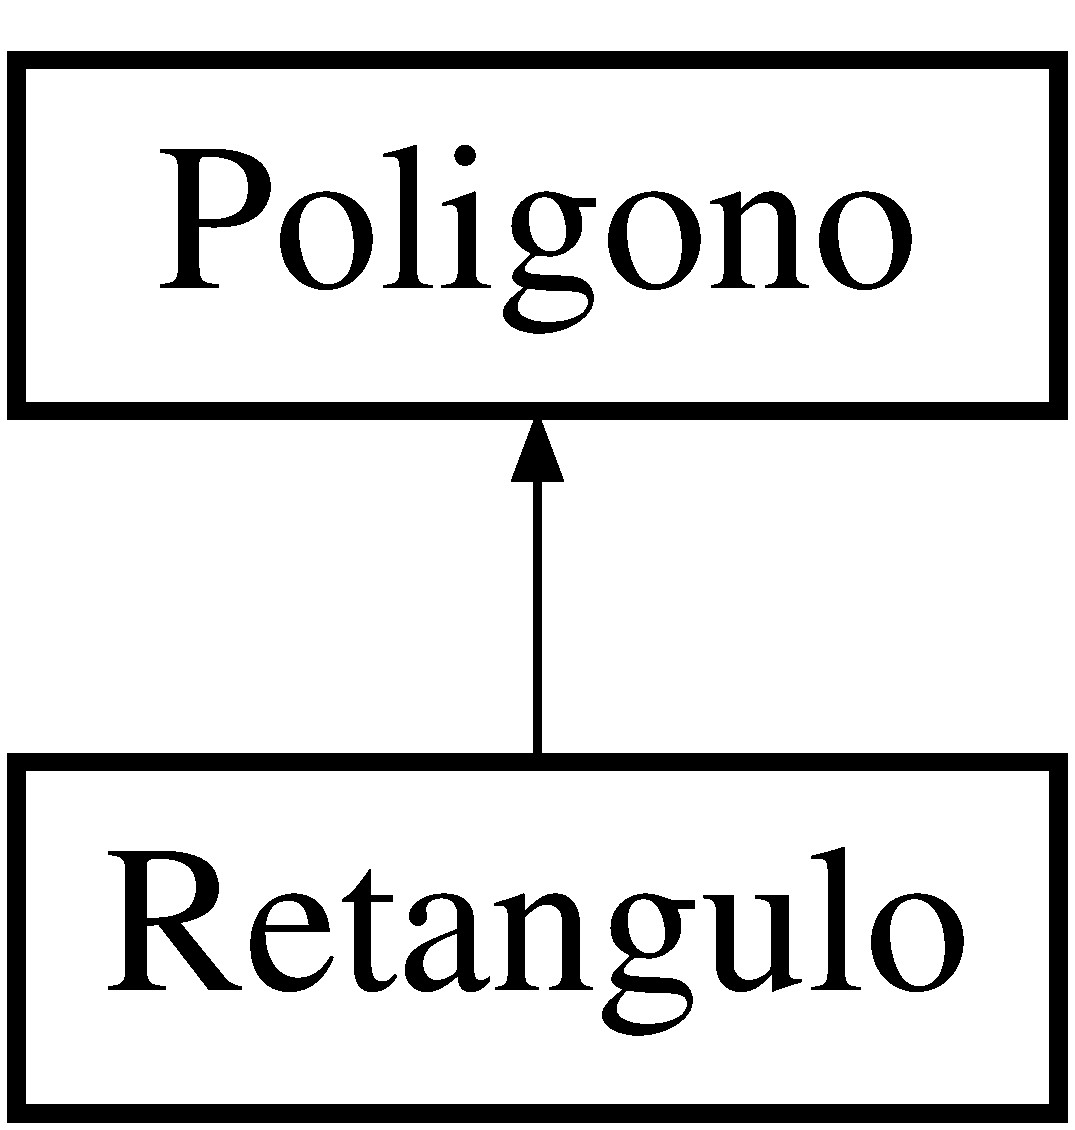
\includegraphics[height=2.000000cm]{class_poligono}
\end{center}
\end{figure}
\subsection*{Membros Públicos}
\begin{DoxyCompactItemize}
\item 
\mbox{\Hypertarget{class_poligono_a9311a9a1496878c09c8508b3636e2870}\label{class_poligono_a9311a9a1496878c09c8508b3636e2870}} 
\mbox{\hyperlink{class_poligono_a9311a9a1496878c09c8508b3636e2870}{Poligono}} ()
\begin{DoxyCompactList}\small\item\em \mbox{\hyperlink{class_poligono}{Poligono}}. \end{DoxyCompactList}\item 
\mbox{\Hypertarget{class_poligono_a4dd7136ee506cb4355cbdc724c55a4a0}\label{class_poligono_a4dd7136ee506cb4355cbdc724c55a4a0}} 
\mbox{\hyperlink{class_poligono_a4dd7136ee506cb4355cbdc724c55a4a0}{$\sim$\+Poligono}} ()
\begin{DoxyCompactList}\small\item\em $\sim$\+Poligono \end{DoxyCompactList}\item 
void \mbox{\hyperlink{class_poligono_aa67788dbd280dd16b3a3f03870844f26}{set\+Vertices}} (float mx, float my)
\begin{DoxyCompactList}\small\item\em set\+Vertices \end{DoxyCompactList}\item 
int \mbox{\hyperlink{class_poligono_a26a3c5ded9660c3389f9a9535700fa5d}{get\+Vertices}} (void)
\begin{DoxyCompactList}\small\item\em get\+Vertices \end{DoxyCompactList}\item 
float \mbox{\hyperlink{class_poligono_a9b7cb6c339f78a5b9432494d8f94816c}{area}} (void)
\begin{DoxyCompactList}\small\item\em area \end{DoxyCompactList}\item 
void \mbox{\hyperlink{class_poligono_adbf605dfd0419b7301c9be0ec1dbe41b}{translada}} (float a, float b)
\begin{DoxyCompactList}\small\item\em translada \end{DoxyCompactList}\item 
void \mbox{\hyperlink{class_poligono_ab50d539e92a775b56c4b70ff52830516}{rotaciona}} (float theta, \mbox{\hyperlink{class_point}{Point}} p, float a, float b)
\begin{DoxyCompactList}\small\item\em rotaciona \end{DoxyCompactList}\item 
\mbox{\Hypertarget{class_poligono_a9e4ab006eceed5bc68d3175127a200e0}\label{class_poligono_a9e4ab006eceed5bc68d3175127a200e0}} 
void \mbox{\hyperlink{class_poligono_a9e4ab006eceed5bc68d3175127a200e0}{imprime}} (void)
\begin{DoxyCompactList}\small\item\em imprime \end{DoxyCompactList}\end{DoxyCompactItemize}


\subsection{Funções membros}
\mbox{\Hypertarget{class_poligono_a9b7cb6c339f78a5b9432494d8f94816c}\label{class_poligono_a9b7cb6c339f78a5b9432494d8f94816c}} 
\index{Poligono@{Poligono}!area@{area}}
\index{area@{area}!Poligono@{Poligono}}
\subsubsection{\texorpdfstring{area()}{area()}}
{\footnotesize\ttfamily float Poligono\+::area (\begin{DoxyParamCaption}\item[{void}]{ }\end{DoxyParamCaption})}



area 

\begin{DoxyReturn}{Retorna}

\end{DoxyReturn}
\mbox{\Hypertarget{class_poligono_a26a3c5ded9660c3389f9a9535700fa5d}\label{class_poligono_a26a3c5ded9660c3389f9a9535700fa5d}} 
\index{Poligono@{Poligono}!get\+Vertices@{get\+Vertices}}
\index{get\+Vertices@{get\+Vertices}!Poligono@{Poligono}}
\subsubsection{\texorpdfstring{get\+Vertices()}{getVertices()}}
{\footnotesize\ttfamily int Poligono\+::get\+Vertices (\begin{DoxyParamCaption}\item[{void}]{ }\end{DoxyParamCaption})}



get\+Vertices 

\begin{DoxyReturn}{Retorna}

\end{DoxyReturn}
\mbox{\Hypertarget{class_poligono_ab50d539e92a775b56c4b70ff52830516}\label{class_poligono_ab50d539e92a775b56c4b70ff52830516}} 
\index{Poligono@{Poligono}!rotaciona@{rotaciona}}
\index{rotaciona@{rotaciona}!Poligono@{Poligono}}
\subsubsection{\texorpdfstring{rotaciona()}{rotaciona()}}
{\footnotesize\ttfamily void Poligono\+::rotaciona (\begin{DoxyParamCaption}\item[{float}]{theta,  }\item[{\mbox{\hyperlink{class_point}{Point}}}]{p,  }\item[{float}]{a,  }\item[{float}]{b }\end{DoxyParamCaption})}



rotaciona 


\begin{DoxyParams}{Parâmetros}
{\em theta} & \\
\hline
{\em p} & \\
\hline
\end{DoxyParams}
\mbox{\Hypertarget{class_poligono_aa67788dbd280dd16b3a3f03870844f26}\label{class_poligono_aa67788dbd280dd16b3a3f03870844f26}} 
\index{Poligono@{Poligono}!set\+Vertices@{set\+Vertices}}
\index{set\+Vertices@{set\+Vertices}!Poligono@{Poligono}}
\subsubsection{\texorpdfstring{set\+Vertices()}{setVertices()}}
{\footnotesize\ttfamily void Poligono\+::set\+Vertices (\begin{DoxyParamCaption}\item[{float}]{mx,  }\item[{float}]{my }\end{DoxyParamCaption})}



set\+Vertices 


\begin{DoxyParams}{Parâmetros}
{\em mx} & \\
\hline
{\em my} & \\
\hline
\end{DoxyParams}
\mbox{\Hypertarget{class_poligono_adbf605dfd0419b7301c9be0ec1dbe41b}\label{class_poligono_adbf605dfd0419b7301c9be0ec1dbe41b}} 
\index{Poligono@{Poligono}!translada@{translada}}
\index{translada@{translada}!Poligono@{Poligono}}
\subsubsection{\texorpdfstring{translada()}{translada()}}
{\footnotesize\ttfamily void Poligono\+::translada (\begin{DoxyParamCaption}\item[{float}]{a,  }\item[{float}]{b }\end{DoxyParamCaption})}



translada 


\begin{DoxyParams}{Parâmetros}
{\em a} & \\
\hline
{\em b} & \\
\hline
\end{DoxyParams}


A documentação para essa classe foi gerada a partir dos seguintes arquivos\+:\begin{DoxyCompactItemize}
\item 
poligono.\+h\item 
poligono.\+cpp\end{DoxyCompactItemize}

\hypertarget{class_retangulo}{}\section{Referência da Classe Retangulo}
\label{class_retangulo}\index{Retangulo@{Retangulo}}
Diagrama de hierarquia para Retangulo\+:\begin{figure}[H]
\begin{center}
\leavevmode
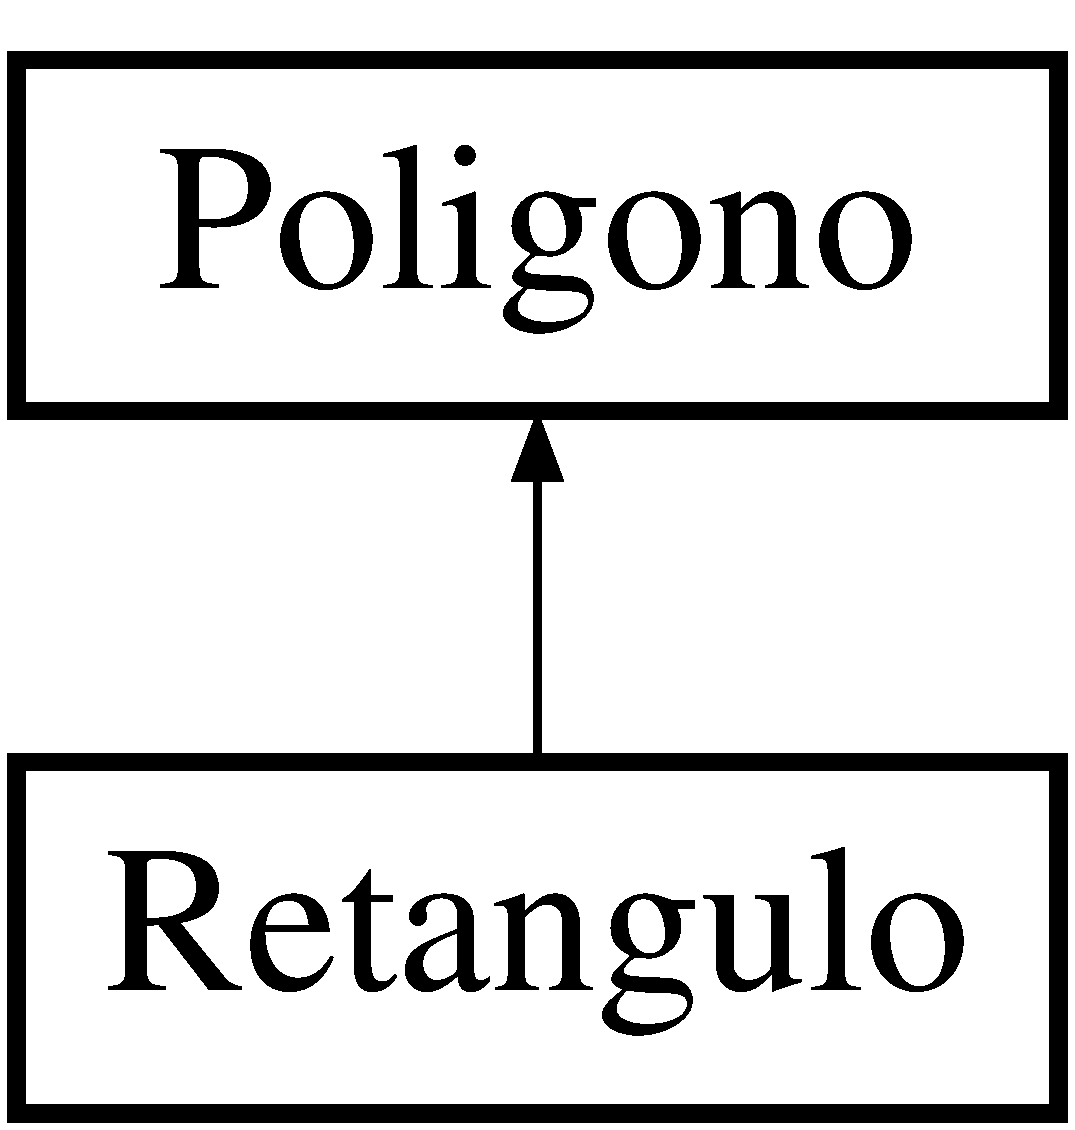
\includegraphics[height=2.000000cm]{class_retangulo}
\end{center}
\end{figure}
\subsection*{Membros Públicos}
\begin{DoxyCompactItemize}
\item 
\mbox{\hyperlink{class_retangulo_acca1dd211eefc8dc04658c943c0d1122}{Retangulo}} (float x, float y, float largura, float altura)
\begin{DoxyCompactList}\small\item\em \mbox{\hyperlink{class_retangulo}{Retangulo}}. \end{DoxyCompactList}\item 
\mbox{\Hypertarget{class_retangulo_a52b1a7f23e13a531a30526825b164615}\label{class_retangulo_a52b1a7f23e13a531a30526825b164615}} 
\mbox{\hyperlink{class_retangulo_a52b1a7f23e13a531a30526825b164615}{$\sim$\+Retangulo}} ()
\begin{DoxyCompactList}\small\item\em $\sim$\+Retangulo \end{DoxyCompactList}\end{DoxyCompactItemize}


\subsection{Construtores e Destrutores}
\mbox{\Hypertarget{class_retangulo_acca1dd211eefc8dc04658c943c0d1122}\label{class_retangulo_acca1dd211eefc8dc04658c943c0d1122}} 
\index{Retangulo@{Retangulo}!Retangulo@{Retangulo}}
\index{Retangulo@{Retangulo}!Retangulo@{Retangulo}}
\subsubsection{\texorpdfstring{Retangulo()}{Retangulo()}}
{\footnotesize\ttfamily Retangulo\+::\+Retangulo (\begin{DoxyParamCaption}\item[{float}]{x,  }\item[{float}]{y,  }\item[{float}]{largura,  }\item[{float}]{altura }\end{DoxyParamCaption})}



\mbox{\hyperlink{class_retangulo}{Retangulo}}. 


\begin{DoxyParams}{Parâmetros}
{\em x} & \\
\hline
{\em y} & \\
\hline
{\em largura} & \\
\hline
{\em altura} & \\
\hline
\end{DoxyParams}


A documentação para essa classe foi gerada a partir dos seguintes arquivos\+:\begin{DoxyCompactItemize}
\item 
retangulo.\+h\item 
retangulo.\+cpp\end{DoxyCompactItemize}

%--- End generated contents ---

% Index
\backmatter
\newpage
\phantomsection
\clearemptydoublepage
\addcontentsline{toc}{chapter}{Sumário}
\printindex

\end{document}
